\section{Storia di Valtara dalla fondazione dell'Impero a
Oggi}\label{storia-di-valtara-dalla-fondazione-dellimpero-a-oggi}

\begin{center}\rule{0.5\linewidth}{0.5pt}\end{center}

\section{I secolo (1-100)}\label{i-secolo-1-100}

\subsection{Anno 1. Fondazione dell'Impero di
Valtara}\label{anno-1.-fondazione-dellimpero-di-valtara}

Fondazione dell'Impero di Valtorria, anche conosciuto come Valtara,
toponimo che ancora oggi viene utilizzato per indicare l'intera regione.
Per la prima volta l'intera Valtara è unificata. Le politiche imperiali
producono l'omogeneità culturale e linguista della regione. Ancora oggi,
nonostante la situazione politica altamente frammentata, il senso di
appartenenza dei popoli di Valtara è forte.

\begin{figure}
\centering
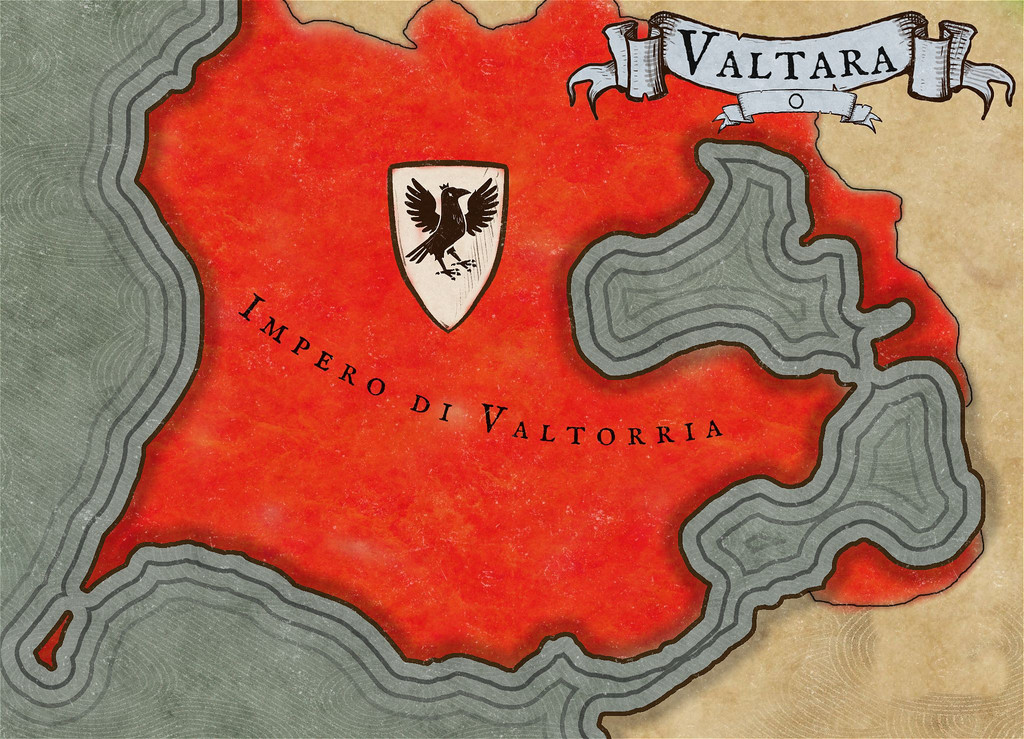
\includegraphics{valtorria_1.jpg}
\caption{valtorria 1.jpg}
\end{figure}

\section{II secolo (101-200)}\label{ii-secolo-101-200}

\section{III secolo (201-300)}\label{iii-secolo-201-300}

\section{IV secolo (301-400)}\label{iv-secolo-301-400}

\section{V secolo (401-500)}\label{v-secolo-401-500}

\section{VI secolo (501-600)}\label{vi-secolo-501-600}

\subsection{Anno 512. La fine dell'Impero di
Valtorria}\label{anno-512.-la-fine-dellimpero-di-valtorria}

I cinquant'anni precedenti alla sua disfatta, avvenuta nel 512 ~furono
segnati da un declino inesorabile, causato da una serie di fattori che
minarono la solidità e la coesione dell'impero.

Le scelte politiche degli ultimi due imperatori furono decisive: in un
tentativo di rafforzare il controllo centrale (in crisi già da tempo),
decisero di concentrare tutte le risorse nella capitale imperiale.

Questa politica centralizzatrice era motivata da diverse ragioni:

\begin{enumerate}
\def\labelenumi{\arabic{enumi}.}
\tightlist
\item
  \textbf{Controllo politico:} Concentrando le risorse nella capitale,
  gli imperatori intendevano aumentare il controllo politico sull'intero
  impero. Centralizzare le decisioni e le risorse significava avere un
  maggiore potere decisionale sulla gestione delle province e degli
  affari interni, permettendo loro di esercitare un controllo più
  diretto sull'amministrazione e sulla politica.
\item
  \textbf{Prestigio e magnificenza:} La capitale, centro del potere e
  della cultura, era spesso vista come il simbolo dell'immagine
  imperiale. Gli imperatori desideravano trasmettere un'immagine di
  grandezza e magnificenza, usando le risorse per ingrandire e adornare
  la città. Questa ostentazione era spesso finalizzata a rafforzare la
  legittimità del loro governo e a impressionare la popolazione e gli
  stati stranieri.
\item
  \textbf{Difesa della capitale:} Negli ultimi anni le minacce interne
  ed esterne aumentarono, ma l'imperatore percepì erroneamente la
  necessità di rafforzare le difese della capitale per garantire la
  sicurezza del governo centrale. Questo portò alla decisione di
  concentrare maggiormente risorse materiali per la costruzione di mura,
  forti e altre infrastrutture difensive, dando il colpo di grazia
  all'economia dell'Impero.
\end{enumerate}

Tuttavia, questa politica di centralizzazione ebbe conseguenze
disastrose, indebolendo le province periferiche e generando un
malcontento diffuso che alla fine portò alla frammentazione dell'impero.
La mancanza di equilibrio tra il potere centrale e le esigenze delle
province rappresentò un fattore chiave nella sua disfatta.

Il malcontento si trasformò in protesta e, nei casi più estremi, in
ribellione. La disaffezione crescente nelle province portò a una
frammentazione dell'Impero di Valtorria nei decenni successivi,
indebolendo progressivamente l'unità dell'Impero.

Parallelamente, la minaccia delle popolazioni settentrionali, nei secoli
precedenti contenuta con abilità, cominciò a mutare da una
preoccupazione costante a un pericolo reale. L'esercito, una volta
formidabile, si ritrovò ad affrontare una crisi senza precedenti.
L'afflusso di reclute si esaurì, poiché la popolazione, impoverita e
trascurata, disertò la chiamata alle armi.

Le tensioni socali esacerbate dalle politiche centralizzatrici portarono
alla desertificazione delle file dell'esercito. La leva obbligatoria,
pensata per garantire la stabilità dello stato, invece minò la sua
forza, trasformando l'esercito da un pilastro di potere a un guscio
vuoto di mercenari, tra cui molti provenienti dallo stesso Nord da cui
arrivava la minaccia.

Le popolazioni nomadi dei Dish, dei Sarat e dei Lout, una volta
confinati ai margini, ora vedevano l'opportunità di penetrare i confini
indeboliti dell'impero per saccheggi e conquiste.

Mentre l'instabilità politica interna minava le fondamenta, le minacce
esterne si moltiplicavano. Le incursioni dei nomadi settentrionali
divennero sempre più insistenti, la pirateria nei mari interni
minacciava i commerci e la sicurezza delle coste. Sebbene l'impero
avesse sempre saputo fronteggiare le minacce con astuzia, in questo
periodo di declino e incertezza, si rivelò incapace di preservare la sua
integrità.

Così, nell'anno 512, l'incubo della caduta dell'Impero si materializzò
in un tragico evento che segnò la fine definitiva di un'era. Gli
attacchi dei pirati, intensificati nei mesi precedenti, raggiunsero il
loro apice quando la flotta dei predoni riuscì a superare le difese
della capitale, attraccando alle porte della città. La loro avanzata fu
spietata, con incursioni notturne e attacchi coordinati che mette in
ginocchio la difesa imperiale. I pirati del capitano INSERIRE NOME
riuscirono ad arrivare a palazzo reale, dove trovarono un imperatore
ormai indifeso che chiedeva pietà. Il capitano INSERIRE NOME mozzò la
testa dell'imperatore e indossò la sua corona, proclamando l'inizio di
un'era dominata dai pirati.

I pirati razziarono la città per un intero anno.

Nel frattempo, le provincie periferiche, già indebolite e disilluse,
videro il loro destino intrecciarsi con quello della capitale. Alcune
furono invase dalle popolazioni del nord, che colsero l'opportunità di
estendere il loro dominio. Altre, stanche della lontananza del potere
centrale, si proclamarono indipendenti, cercando rifugio in una
autonomia che sembrava promettere una speranza di stabilità.

Così, l'Impero di Valtorria, una volta potente, cadde in un turbine di
violenza e anarchia. L'inizio della ``grande era dei pirati'' (che noi
oggi identifichiamo come Prima Era Pirata) fu proclamato tra le rovine
di ciò che era stato un grande impero, e il destino delle provincie fu
segnato da una frammentazione che avrebbe definito il corso della storia
per gli anni a venire.

Il sesto secolo è stato definito dagli storici come ``\textbf{il secolo
delle razzie}''.

Nei successivi cento anni dalla caduta dell'impero, i territori
valtaresi furono continuo teatro di sanguinose lotte e scontri
incessanti.

Le popolazioni settentrionali, affamate di potere e risorse,
continuarono a riversarsi nella penisola, saccheggiando le più grandi
città, e stabilendosi permanentemente nelle vallate. La geografia
dell'antico impero fu ridisegnata dai conflitti, con nuovi regni che
sorgevano e crollavano nell'arco di un solo anno.

Nel Sud Valtara, gli ultimi lealisti all'ormai defunto impero si unirono
per formare una Lega. Questa coalizione di signori, ancora legati ai
valori e alle tradizioni dell'antico regime, si oppose con fermezza agli
invasori del nord. Le terre del Sud Valtara divennero l'ultimo baluardo
di stabilità, un rifugio per coloro che cercavano riparo dalla tempesta
che infuriava oltre i loro confini.

I Ducati Meridionali di Valtara resistettero con tenacia, consolidando
le proprie difese.

\subsection{\texorpdfstring{Anno 578. \textbf{Prima era dei Pirati:
fondazione della Repubblica dei
Pirati}}{Anno 578. Prima era dei Pirati: fondazione della Repubblica dei Pirati}}\label{anno-578.-prima-era-dei-pirati-fondazione-della-repubblica-dei-pirati}

Nel 578, i pirati erano tanto potenti nei mari interni da fondarono una
repubblica. Fondata da un consiglio composto dai più spietati e
influenti pirati dell'epoca, che utilizzarono il termine ``repubblica''
per indicare erroneamente un territorio libero e anarchico. Nessuno però
prese la responsabilità di amministrare i territori della neonata
repubblica, che di fatto non era altro che un insieme di territori,
divisi dal mare, in cui l'unica regola era quella del più forte.
Nonostante l'intento iniziale di creare una società basata sulla
libertà, l'assenza di una figura di autorità portò a una competizione
sfrenata tra i pirati. Molti capitani, desiderosi di accrescere il
proprio potere, si autoproclamarono ``Re della Repubblica dei Pirati''.
Ciò scatenò conflitti interni, che portarono alla disfatta della
repubblica in soli 30 anni. Nonostante il fallimento di questo
esperimento di governo, la Repubblica dei Pirati rappresentò il culmine
della Prima Era dei Pirati

\begin{figure}
\centering
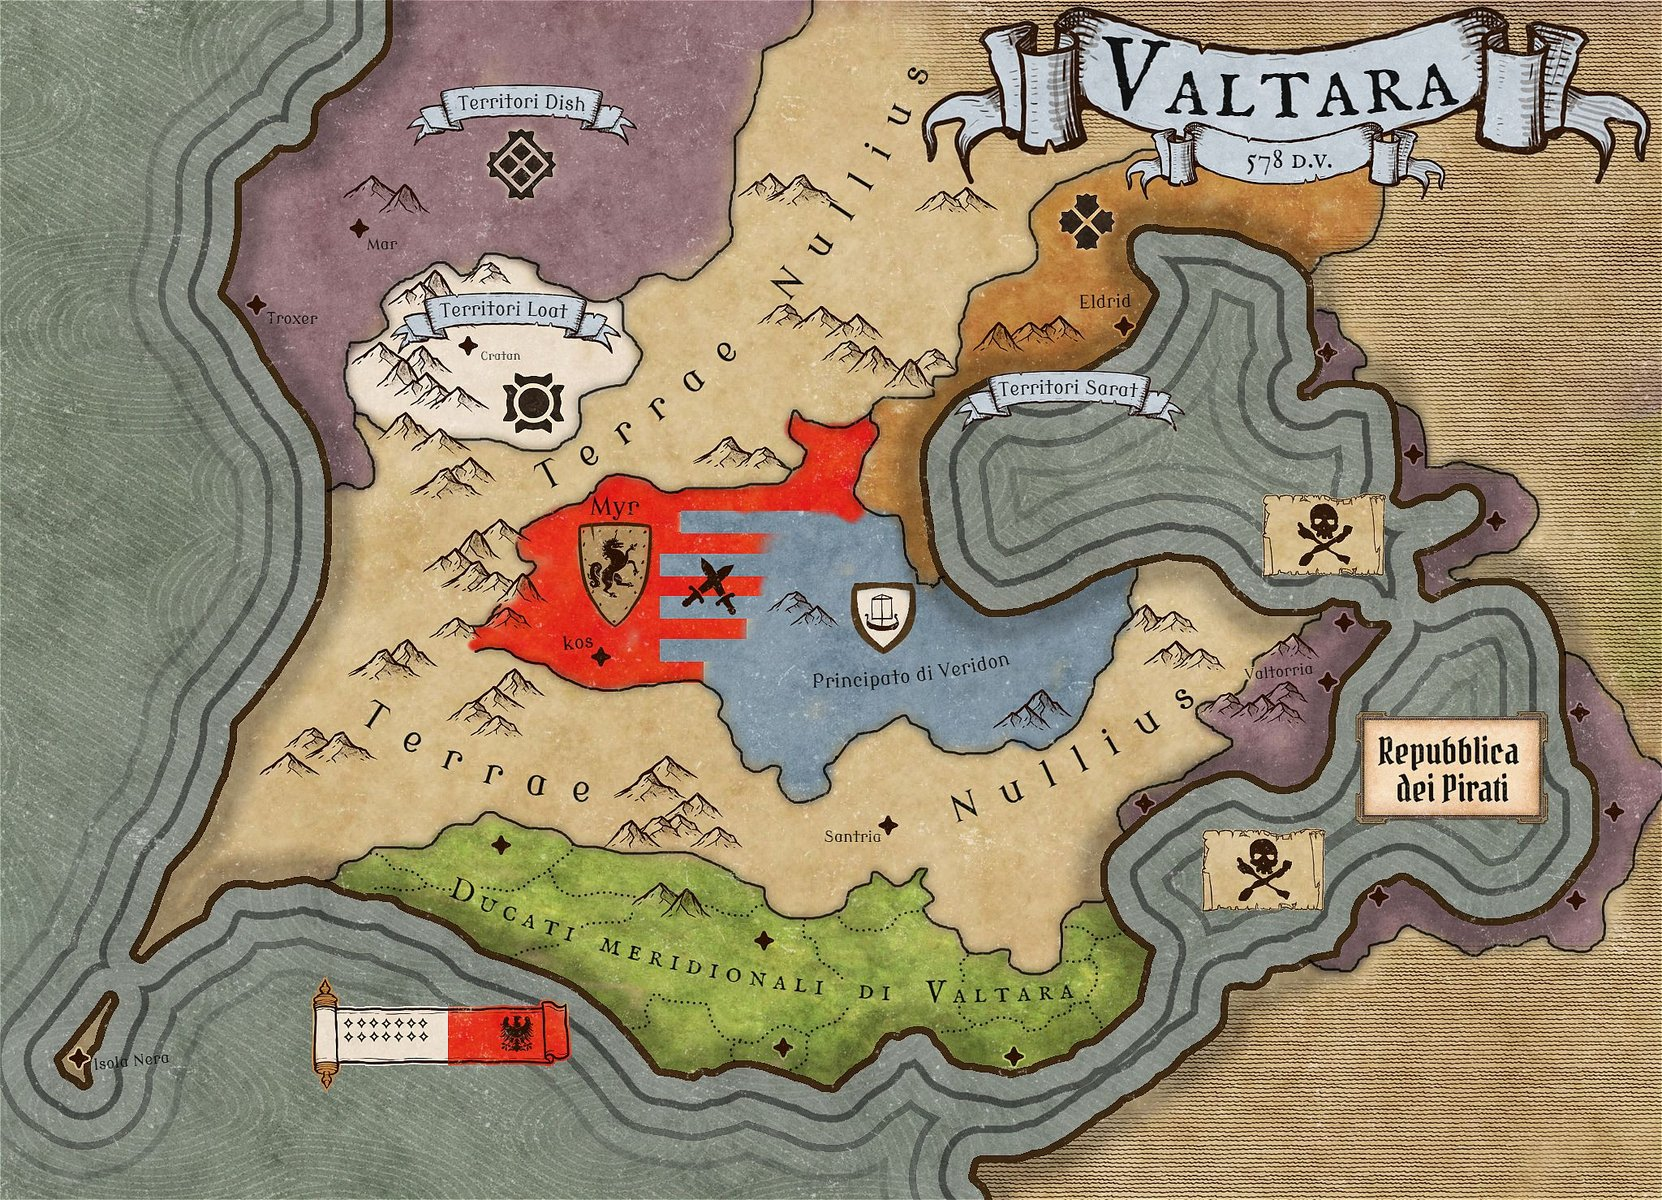
\includegraphics{Valtorria_578.jpg}
\caption{Valtorria 578.jpg}
\end{figure}

\section{VII secolo (601-700)}\label{vii-secolo-601-700}

\subsection{Anno 650 Nuovi Regni, nuovi
equilibri}\label{anno-650-nuovi-regni-nuovi-equilibri}

La carta geografica di Valtara continua a mutare: le popolazioni di
razziatori dal nord si stabiliscono nelle regioni settentrionali della
penisola, dove nascono potenti regni come quello Dishartiano, ancora
oggi grande e potente, quello Sarat, e quello dei Territori Liberati di
Avaloria (da ``Ava lor'' letteralmente ``Vento Celeste'' in dishartano
antico).

\begin{figure}
\centering
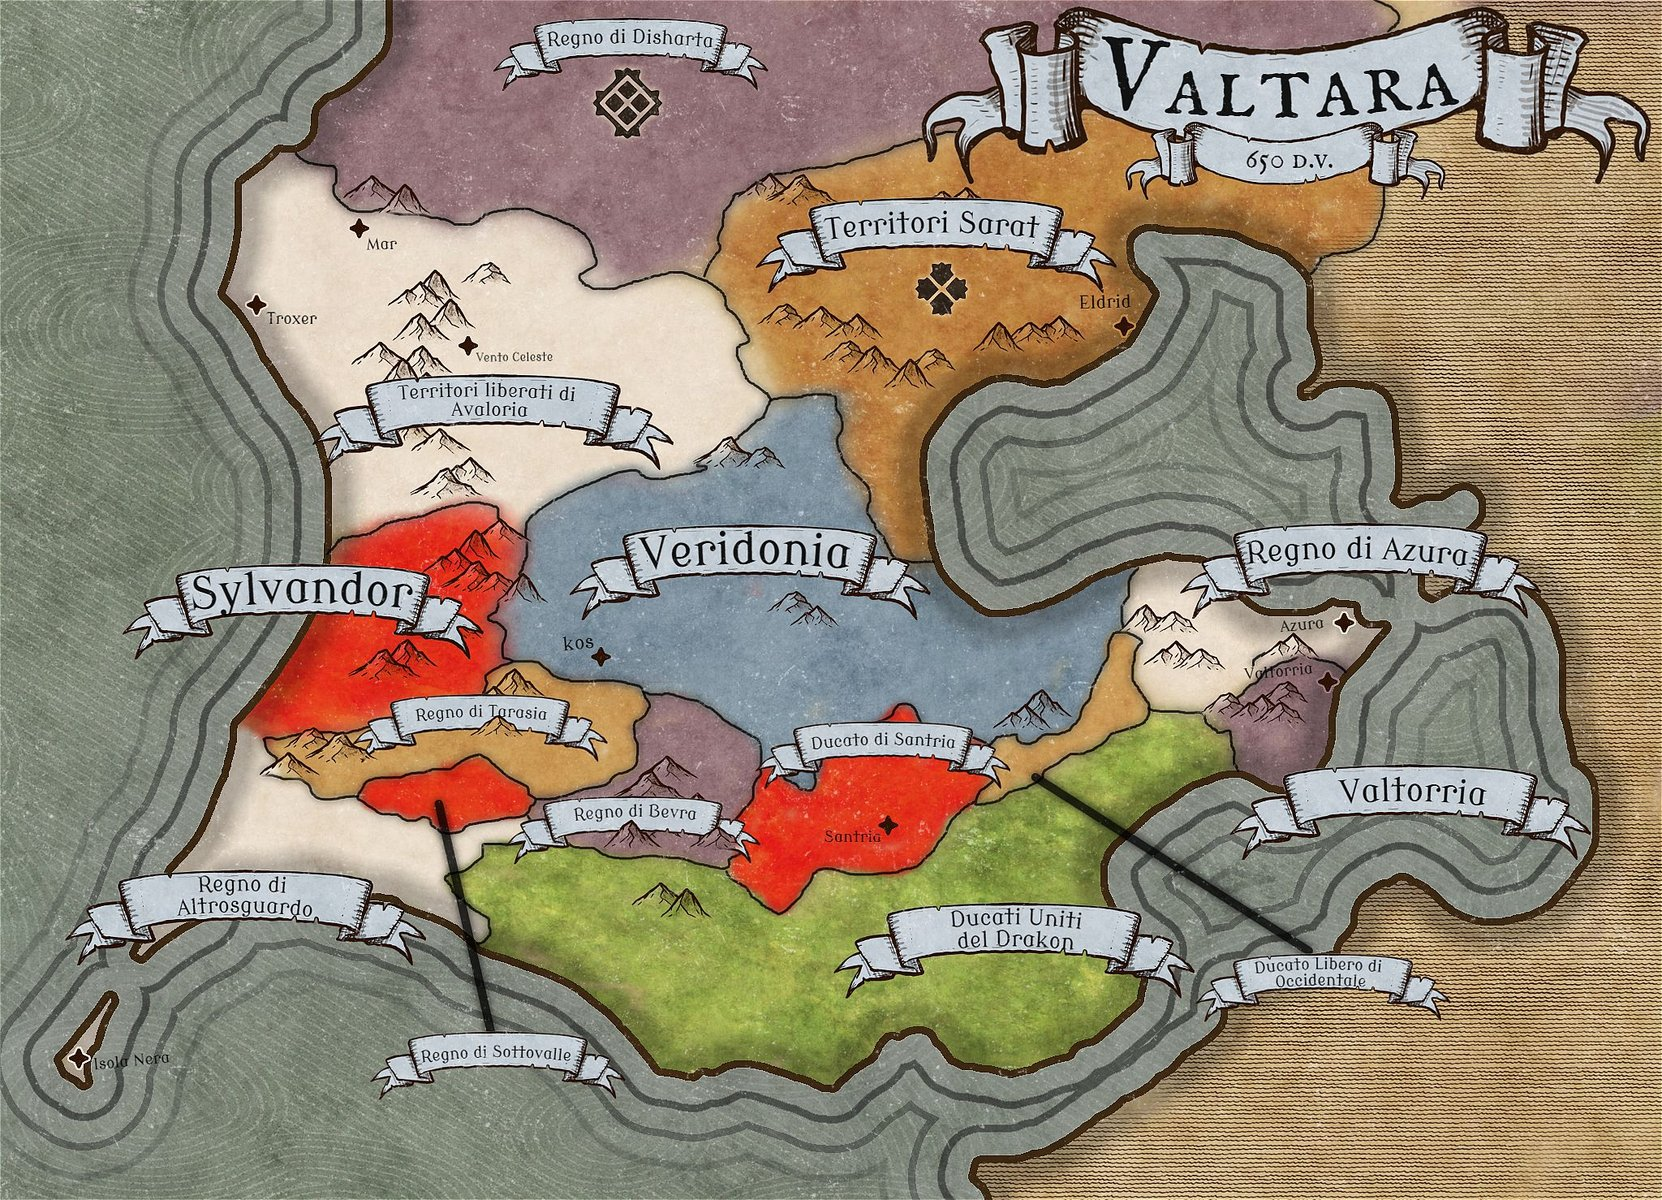
\includegraphics{Valtorria_650.jpg}
\caption{Valtorria 650.jpg}
\end{figure}

A sud, i Ducati Meridionali accrescono il proprio potere e influenza,
trasformando la loro alleanza in un vero e proprio stato federale, i
Ducati Uniti del Drakondor. Il nuovo stato continuerà ad annettere nuovi
territori a Nord e ad Est fino ai primi anni dell'ottavo secolo, quando
i Ducati Uniti diventeranno il potente Drakodor. In tutto il resto della
penisola nuovi ducati si proclamano indipendenti, nascono regni come
quello di Veridonia, che vedrà però una drastica riduzione dei propri
territori a causa dei moti espansionistici dei vicini. Guerre e continue
annessione continuano a modificare la geografia politica valtarese.
Dovremo aspettare il secolo successivo per la stabilità politica della
regione.

\section{VIII secolo (701-800)}\label{viii-secolo-701-800}

\subsection{Anno 712. I regni degli
Eredi}\label{anno-712.-i-regni-degli-eredi}

Nel 712, dopo esattamente 200 anni dalla disfatta dell'impero, la
penisola Valtarese viene divisa da 5 regni, guidati tutti da dinastie
che si dicono essere dirette discendenti della famiglia imperiale di
Valtorria.

\begin{figure}
\centering
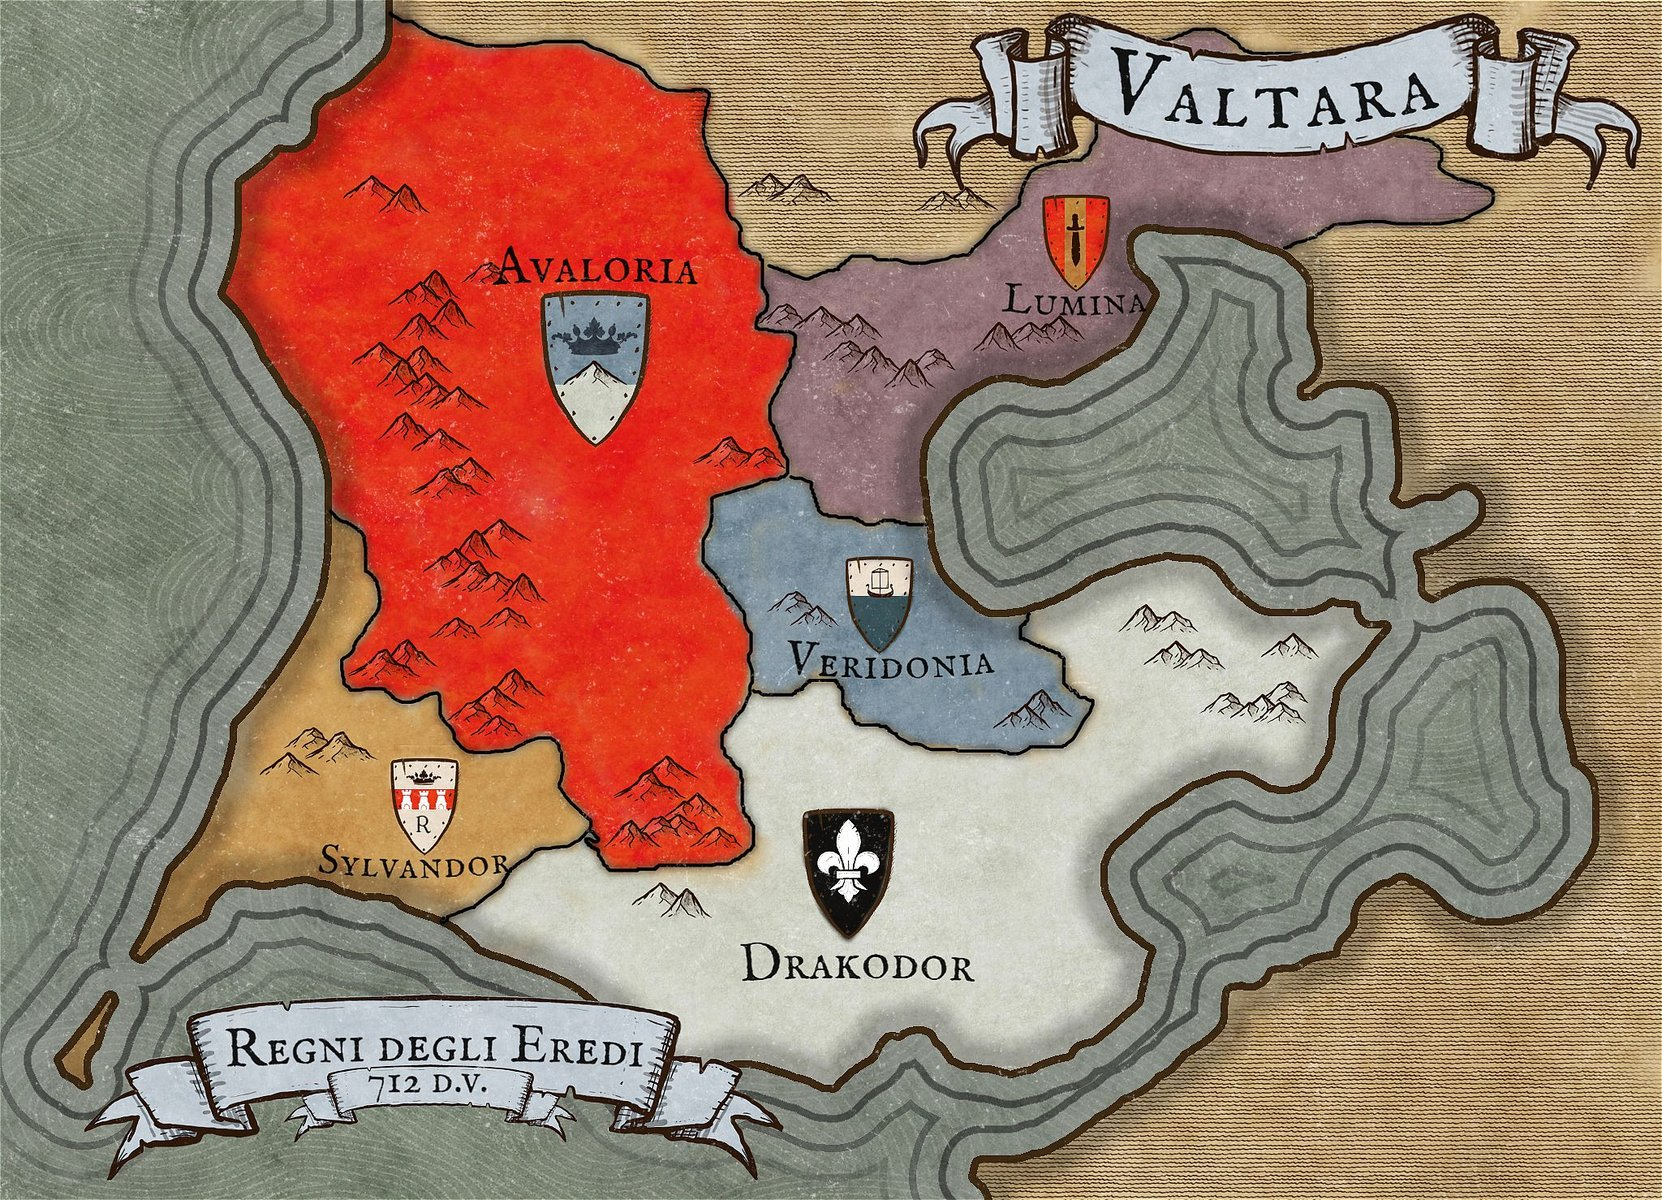
\includegraphics{Valtorria_712.jpg}
\caption{Valtorria 712.jpg}
\end{figure}

\textbf{Veridonia}: il regno è il più antico dei 5. Nato subito dopo la
caduta dell'impero come Principato di Veridon, poiché governato dal
diretto discendente dell'imperatore. Il regno sopravvisse alle invasioni
del nord, e crebbe per più di un secolo annettendo poco a poco i
territori limitrofi. Con l'inizio dell'Ottavo secolo, tuttavia, i
territori del Veridon verranno presi di mira dall'espansione dei regni
vicini, portando i confini dell'antico principato a restringersi.

\textbf{Drakodor}: Anche questo regno deve la sua nascita alla caduta
dell'impero. Inizialmente alleanza tra ducati delle regioni meridionali
di Valtara, nel corso di 2 secoli accrebbe il proprio potere,
espandendosi fino ad annettere i territori dell'antica capitale.
Diventata una monarchia a inizio dell'Ottavo Secolo, vide salire al
trono il duca di Valtorria, che vantava discendenze imperiali.

\textbf{Sylvandor}: Regno nato proprio nel 712, dall'unione dei
territori del Sylvandor con il regno di Altrosguardo a seguito di un
matrimonio.

\textbf{Avaloria}: Regno nato a seguito dell'occupazione della
Nortandria da parte dei Loat, che proclamarono Vento Celeste (Ava Lor in
dishartano antico) come loro capitale. Il regno crebbe nei secoli,
estendendo i suoi confini a Nord e a Sud, occupando quasi per intero la
catena montuosa della Sila, e buona parte della Foresta dei Giganti.

\textbf{Lumina}: Unica repubblica di Valtara, nasce a inizio dell'Ottavo
secolo, dopo una rivolta delle popolazioni del Mitegardiane contro i
Sarat, che per 2 secoli avevano occupato e governato la regione. Dopo la
cattura del re e la sua decapitazione pubblica, viene proclamata la
repubblica di Lumina (da Lumih, ovvero Libertà in dishartano antico).

Tutti e 5 i regni sono destinati a sopravvivere dopo l'anno 1000,
influenzando per 3 secoli la politica della regione.

\section{XI secolo (801-900)}\label{xi-secolo-801-900}

\section{X secolo (901-1000)}\label{x-secolo-901-1000}

\section{XI secolo (1001-1100)}\label{xi-secolo-1001-1100}

\subsection{Anno 1032. La Piaga}\label{anno-1032.-la-piaga}

Una forte crisi climatica mette in ginocchio l'intera regione. Diverse
specie vegetali si ammalano e i campi non sono più produttivi. La crisi
economica sgretola molte tra le autorità statali e la popolazione viene
decimata dalle malattie

\subsection{Anno 1086. Terre Libere e
aride}\label{anno-1086.-terre-libere-e-aride}

La Piaga, un fenomeno devastante che ha scosso le regioni centrali e
meridionali di Valtara e della penisola di Medina in un arco temporale
di poco più di cinquant'anni, ha lasciato un'impronta indelebile nella
storia di quei luoghi. La sua influenza ha avuto ripercussioni dirette
sull'assetto economico e politico dei regni coinvolti.

La crisi agricola, innescata principalmente dalle difficoltà incontrate
nelle grandi pianure del Drakon e nella regione della Foresta dei
Giganti, ha portato al crollo dell'economia dei regni del Drakodor e di
Avaloria. Nel Drakodor, l'unità politica è stata messa in discussione
mentre la popolazione ha subito pesantemente le conseguenze della
carestia e delle malattie. Le città sono state abbandonate e ciò che un
tempo era un regno prospero è diventato un deserto.

Anche Veridonia e Avaloria hanno vissuto esperienze simili, sebbene
Avaloria abbia reagito in modo più efficace alla crisi. Tuttavia,
nonostante gli sforzi, l'indebolimento economico ha reso il regno
vulnerabile all'invasione Dishartana, che ha sfruttato la situazione a
proprio vantaggio.

Le regioni settentrionali, sebbene non completamente immuni, hanno
subito minori conseguenze rispetto alle regioni centrali e meridionali.
La Repubblica di Lumina, al contrario, ha approfittato della crisi per
espandere il proprio potere e territorio, annettendo aree
strategicamente importanti per il commercio marittimo lungo le coste di
Valtara e Medina.

Nonostante le avversità, il Regno di Sylvandor è riuscito a resistere e
addirittura ad ampliare i propri confini, recuperando territori
precedentemente persi a Nord, a seguito dell'espansione del regno di
Avaloria.

\begin{figure}
\centering
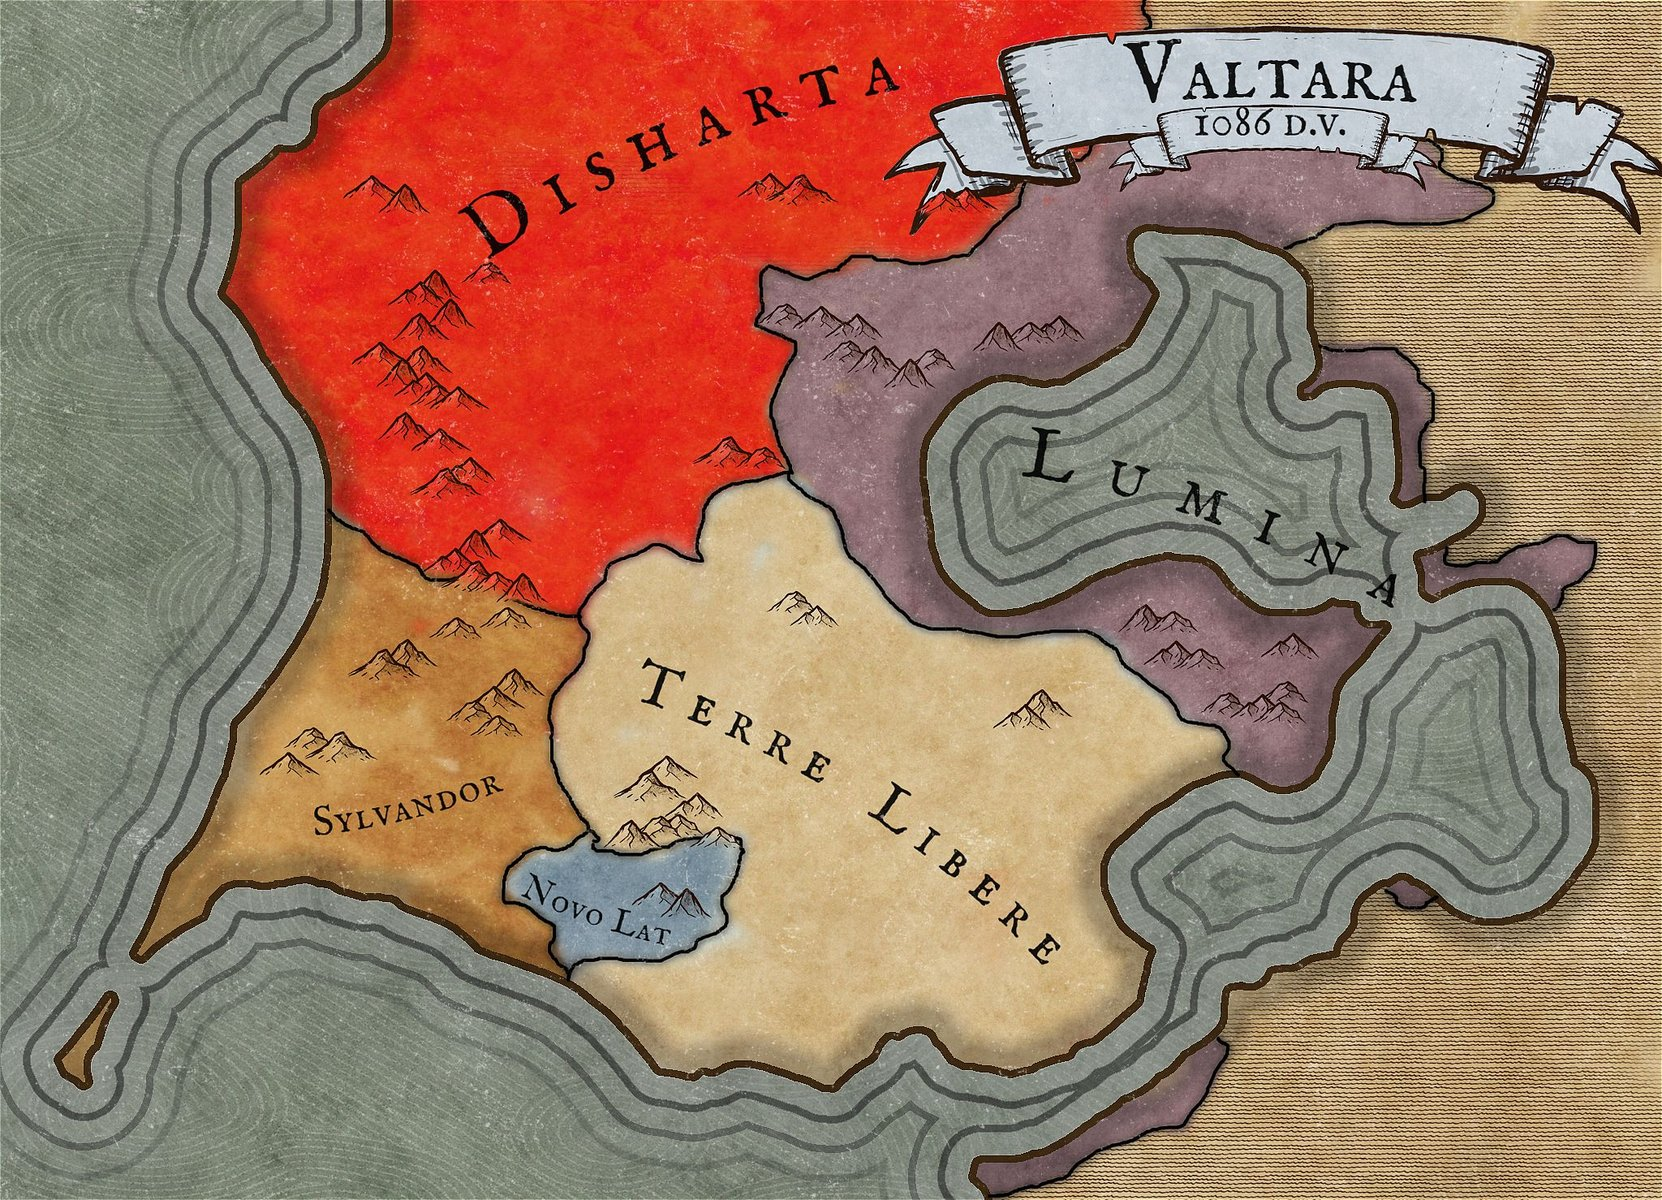
\includegraphics{1086.jpg}
\caption{1086.jpg}
\end{figure}

Molti territori Valtaresi rimasero al di fuori di alcun controllo
territoriale. Per la prima volta nella storia di Valtara si inizia a
parlare di Terre Libere con riferimento a luoghi indipendenti non
controllati da entità statali di vario genere.

\section{XII secolo (1101-1200)}\label{xii-secolo-1101-1200}

\section{XIII secolo (1201-1300)}\label{xiii-secolo-1201-1300}

\subsection{Anno 1237. Secolo di
migrazioni}\label{anno-1237.-secolo-di-migrazioni}

La piaga era ormai lontana, e Valtara, nei due secoli dall'inizio della
crisi, si riprese notevolmente. Le terre nel cuore della regione
rimasero libere, ma nuovi regni sorgevano sulle coste, dove i continui
commerci e le terre più fertili permisero una più rapida ripresa,

Se da una parte la penisola Valtariana sperimentava una notevole
ripresa, non si poteva dire lo stesso per l'isolata isola di Rotrekia.
Lì, la crisi persisteva e la povertà dilagava, spingendo alcune
popolazioni a cercare una nuova vita oltre i confini dell'isola. Le onde
migratorie da Rotrekia verso il Sud di Valtara non portarono solo
speranze di un futuro migliore, ma anche tensioni e conflitti con i
regni già insediati nella zona.

Conosciuti come gli Alisei dalle popolazioni autoctone, questi migranti
si stabilirono sulle coste meridionali di Valtara. Proprio in queste
regioni si erano formati nuovi regni, rigenerati più rapidamente grazie
ai fiorenti commerci marittimi. Tuttavia, gli Alisei trovarono
resistenza al loro arrivo e decisero di espandere i loro insediamenti
verso le coste del Novo Lat e del Sylvandor.

Per circa due secoli a venire, le popolazioni provenienti da Rotrekia,
in costante flusso migratorio, combatterono con i regni del Sud per
conquistare un pezzo di terra che potessero chiamare casa. Le coste
diventarono il teatro di scontri e tensioni mentre le popolazioni
autoctone e gli Alisei lottavano per la supremazia e il controllo delle
risorse.

Questo periodo di conflitti e migrazioni avrebbe segnato profondamente
la storia delle terre meridionali di Valtara, plasmando le dinamiche
politiche e sociali per generazioni a venire.

\begin{figure}
\centering
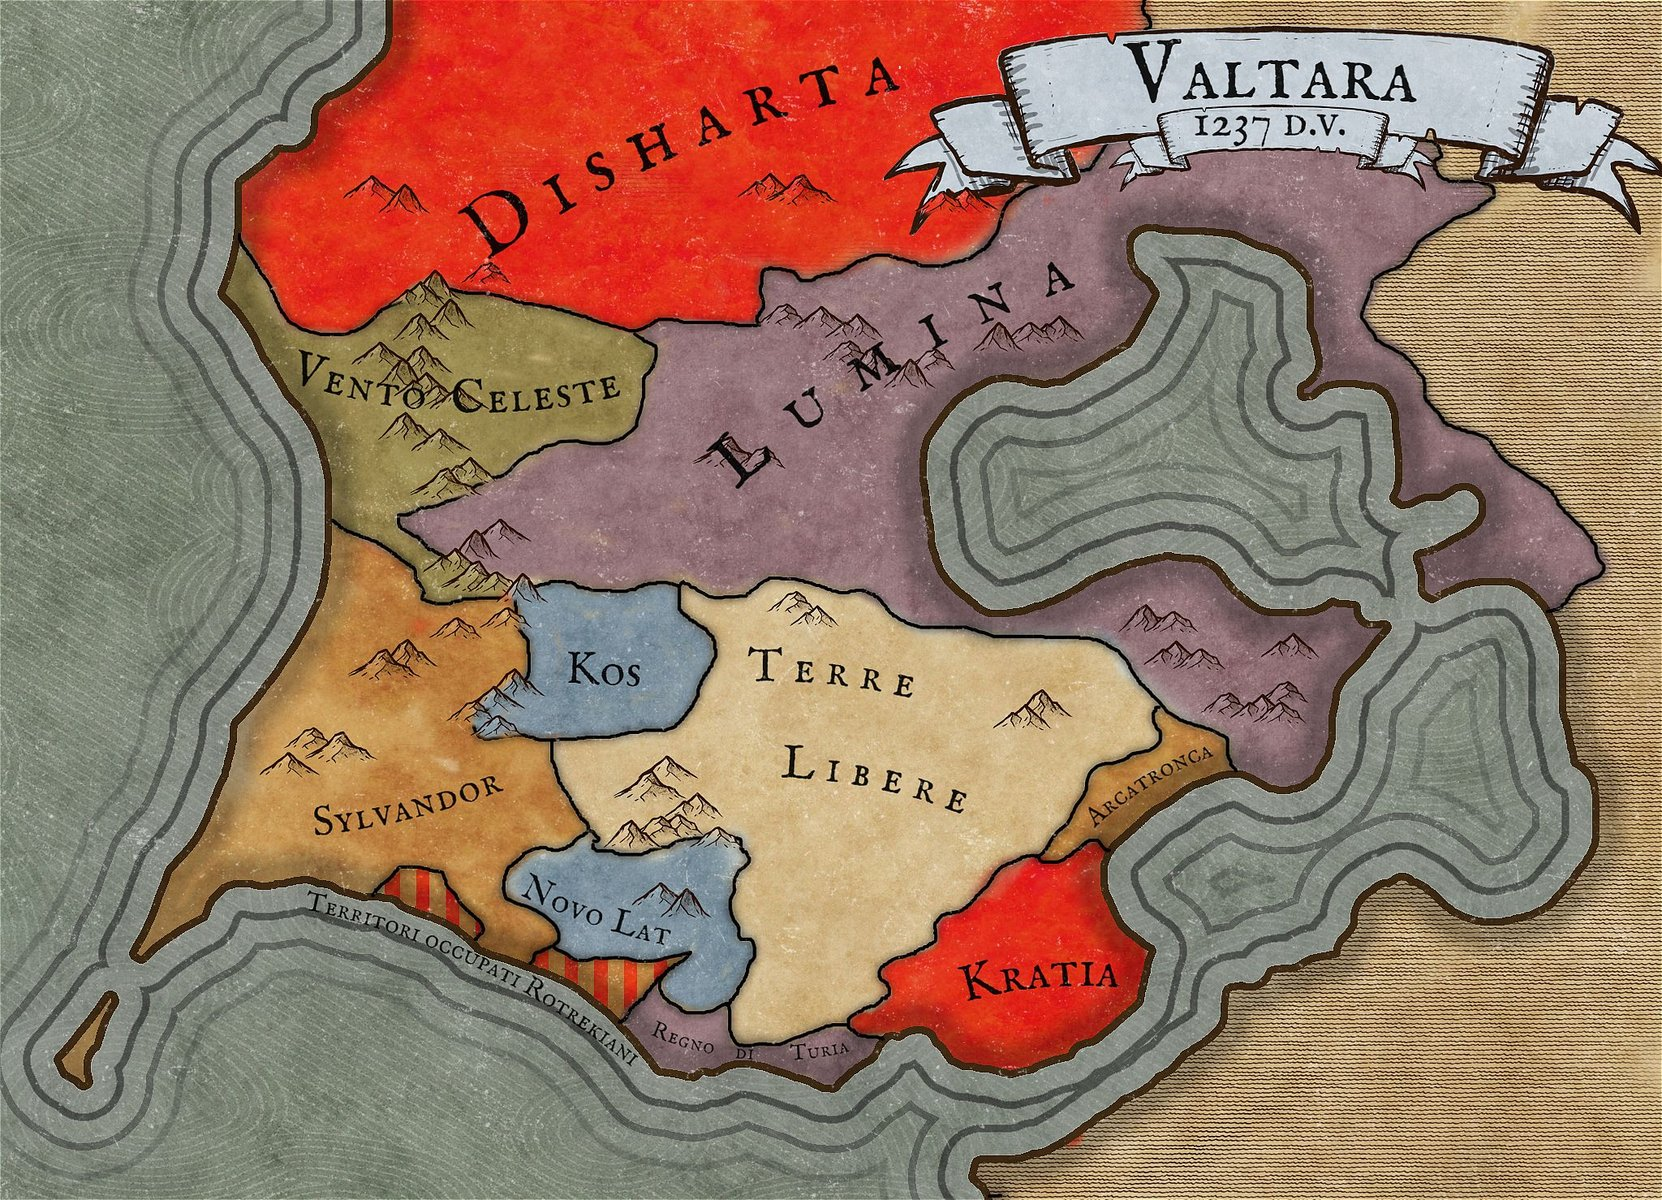
\includegraphics{1200_veea.jpg}
\caption{1200 veea.jpg}
\end{figure}

Nel frattempo, a nord della penisola, la situazione era giunta a un
punto critico. I territori occupati dal regno di Disharta erano in
fermento, con il malcontento che dilagava tra la popolazione oppressa. I
signori di Vento Celeste e di Kos, vedendo l'opportunità di liberare i
propri territori, decisero di stringere un'alleanza con la potente
Repubblica di Lumina.

Il patto tra le due città settentrionali e Lumina era chiaro: la
repubblica avrebbe fornito supporto bellico per liberare i territori
dalle grinfie di Disharta. L'obiettivo primario era spingere più a nord
possibile i confini dell'occupante. In cambio del suo aiuto, Lumina
avrebbe ottenuto il controllo di tutti i territori liberati, ad
eccezione di quelli che facevano parte delle provincie di Vento Celeste
e Kos.

L'accordo fu siglato e la guerra ebbe inizio. Anni di scontri e
battaglie si susseguirono mentre le forze alleate avanzavano verso il
nord, combattendo contro le truppe dishartiane e riconquistando
territorio dopo territorio. Lumina, con la sua potenza economica e
militare, garantiva un supporto cruciale alle città ribelli.

La guerra perdurò per anni, ma alla fine l'ostinazione e la
determinazione delle forze alleate portarono alla vittoria. I territori
di Lumina si ingrossarono considerevolmente, mentre Vento Celeste e Kos
ottennero finalmente l'indipendenza tanto agognata.

\section{XIV secolo (1301-1400)}\label{xiv-secolo-1301-1400}

\section{XV secolo (1401-1500)}\label{xv-secolo-1401-1500}

\subsection{Anno 1415 Fondazione del Regno degli
Alisei}\label{anno-1415-fondazione-del-regno-degli-alisei}

Dopo l'ultimo grande flusso migratorio nel 1378, le popolazioni
provenienti dall'isola di Rotrekia continuarono a cercare rifugio sulle
coste meridionali di Valtara, mescolandosi con le comunità già
insediate.

in 200 anni di convivenza furono diversi gli accordi che gli Alisei
stipularono e molte le battaglie che dovettero affrontare. Nel 1397 ad
esempio, il Novo Lat permetteva ad alcune comunità Rotrekiane di
stabilirsi permanentemente in alcune zone disabitate del suo territorio.
Questo accordo doveva stabilire una pace tra le due nazioni, e
funzionare da base per la convivenza. 10 anni dopo salì al trono del
Novo Lat un nuovo sovrano che vedeva i rotrekiani, a differenza del suo
predecessore, come una minaccia per la stabilità del regno. Nel 1412
ordinò di distruggere ogni segno del passaggio dei rotrekiani nel regno,
i villaggi furono bruciati e i suoi abitanti trucidati. Scoppiò la
guerra tra le due nazioni, che si concluse con la caduta del Novo Lat
cadde nel 1414, dopo una violenta invasione da parte degli Alisei.
L'invasione portò alla fondazione del Regno di Alisgan, un'entità
politica emergente che avrebbe avuto un impatto significativo sulla
regione.

Gli accordi tra Alisgan e il Sylvandor furono cruciali per consolidare
la posizione del nuovo regno. Alisgan promise di non continuare con la
sua espansione territoriale in cambio del ripristino delle vie
commerciali orientali da parte del Sylvandor. Questo accordo, sebbene
precario, contribuì a stabilizzare la regione e a garantire una certa
stabilità politica e economica per entrambi i regni.

La fondazione di Alisgan rappresentava non solo l'affermazione di una
nuova entità politica, ma anche la continuazione di un processo di
trasformazione e adattamento che aveva caratterizzato la storia delle
terre meridionali di Valtara. Nel corso dei secoli a venire, il Regno di
Alisgan avrebbe giocato un ruolo sempre più importante nella politica e
nella cultura della regione, lasciando un'impronta indelebile nella
storia di Valtara.

\begin{figure}
\centering
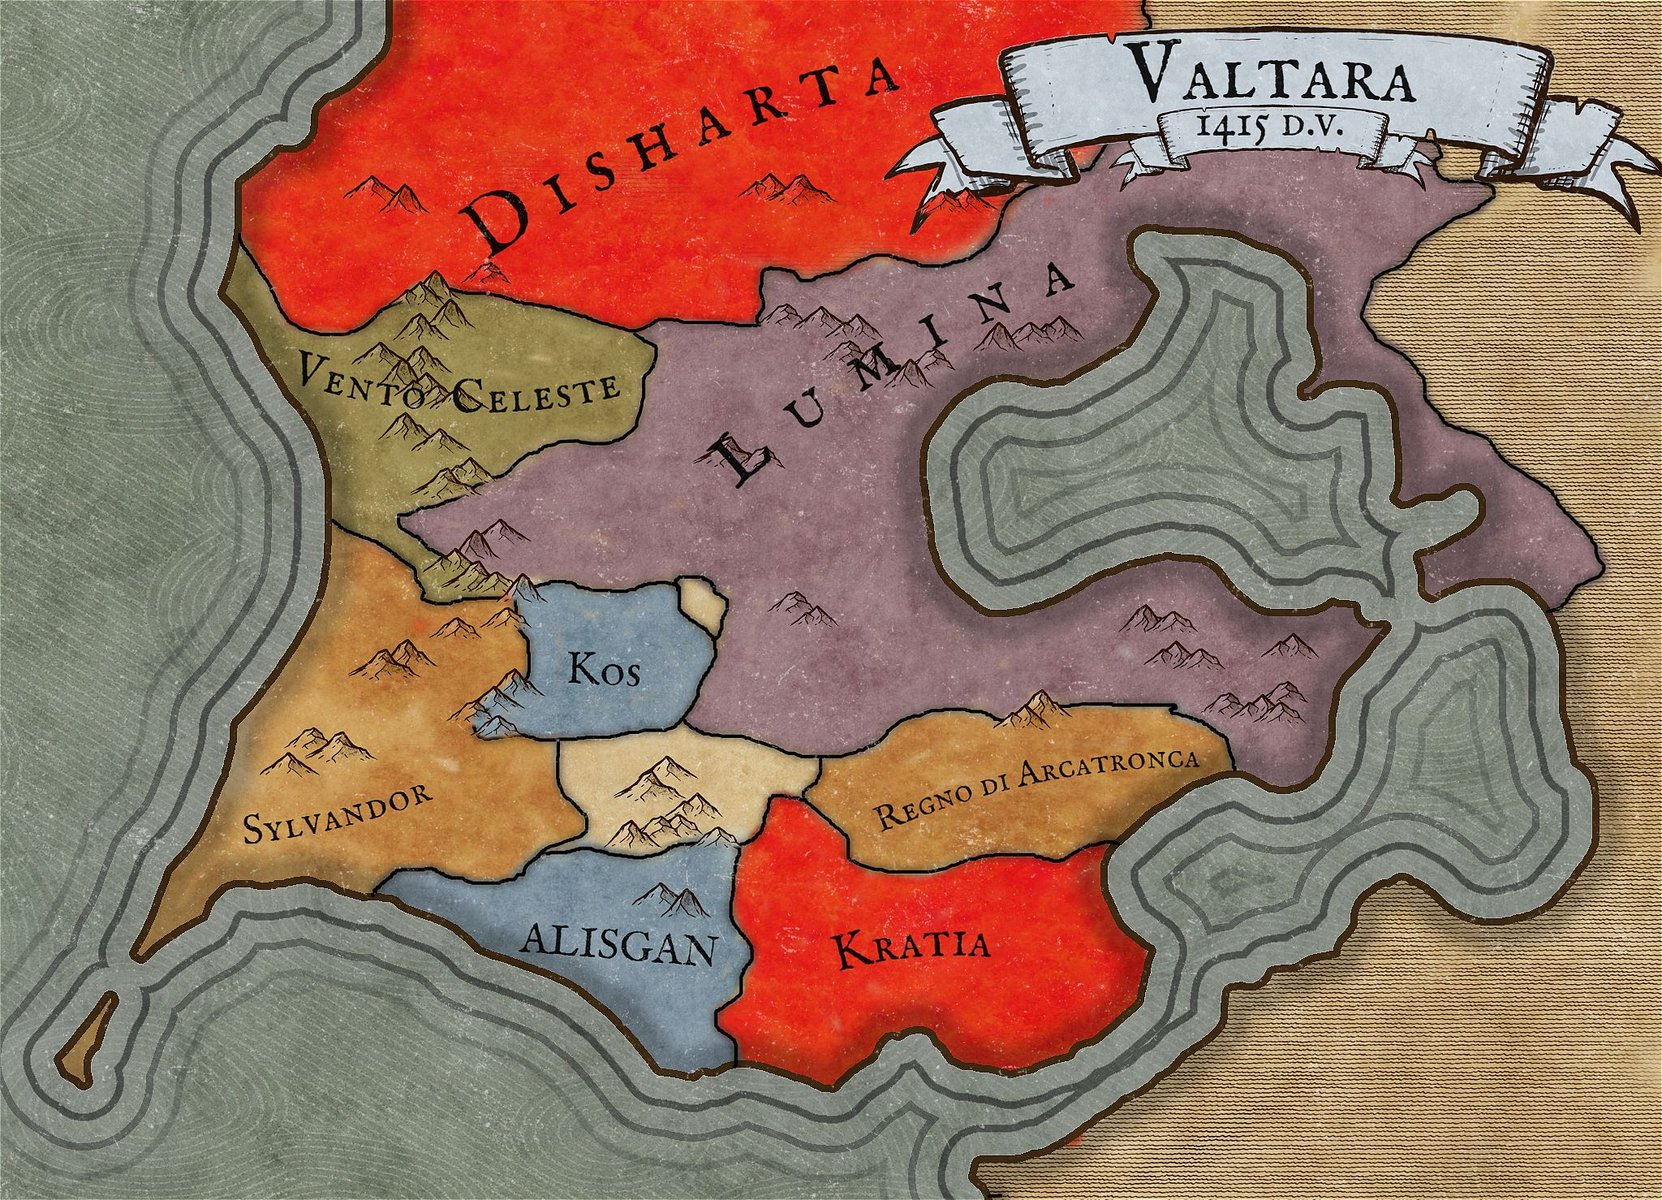
\includegraphics{dfbbd.jpg}
\caption{dfbbd.jpg}
\end{figure}

Mentre il Regno di Alisgan consolidava il suo potere sulle coste
meridionali di Valtara, gli altri regni della regione vedevano un
periodo di crescita economica. I regni si trovavano ad affrontare una
competizione feroce per il controllo delle terre libere. Il controllo
del territorio non era solo una questione di sicurezza e risorse, ma
anche un simbolo di potenza per gli stati. Di conseguenza, le terre
libere divennero teatro di scontri e conflitti mentre i regni cercavano
di estendere il proprio dominio e consolidare la propria posizione nella
regione.

\section{XVI secolo (1501-1600)}\label{xvi-secolo-1501-1600}

\subsection{Anno 1557. Fondazione del regno di
Isauria}\label{anno-1557.-fondazione-del-regno-di-isauria}

La potente Repubblica di Lumina perde gran parte dei suoi territori
oltre i mari interni, segnando l'inizio del declino della più influente
potenza della regione.

La perdita di territori oltre i mari interni fu il risultato di una
serie di eventi che minarono la stabilità e l'autorità della Repubblica
di Lumina. Tra questi, uno degli avvenimenti più significativi fu la
proclamazione di indipendenza dei territori sulle coste settentrionali
di Medina, che diede vita al nuovo stato di Isauria.

La nascita di questo nuovo stato non solo ridimensionò l'influenza nei
mari di Lumina, ma anche riorientò gli equilibri di potere tra gli stati
confinanti.

Il declino di Lumina e l'emergere di Isauria come un nuovo attore
politico e territoriale nella regione avrebbero avuto ripercussioni
significative sul futuro di Valtara e delle terre circostanti.

\section{XVII secolo (1601-1700)}\label{xvii-secolo-1601-1700}

\section{XVIII secolo (1701-1800)}\label{xviii-secolo-1701-1800}

\section{XIX secolo (1801-1900)}\label{xix-secolo-1801-1900}

\section{XX secolo (1901-2000)}\label{xx-secolo-1901-2000}

\section{XXI secolo (2001-2100)}\label{xxi-secolo-2001-2100}

\subsection{Anno 2023}\label{anno-2023}

\begin{figure}
\centering
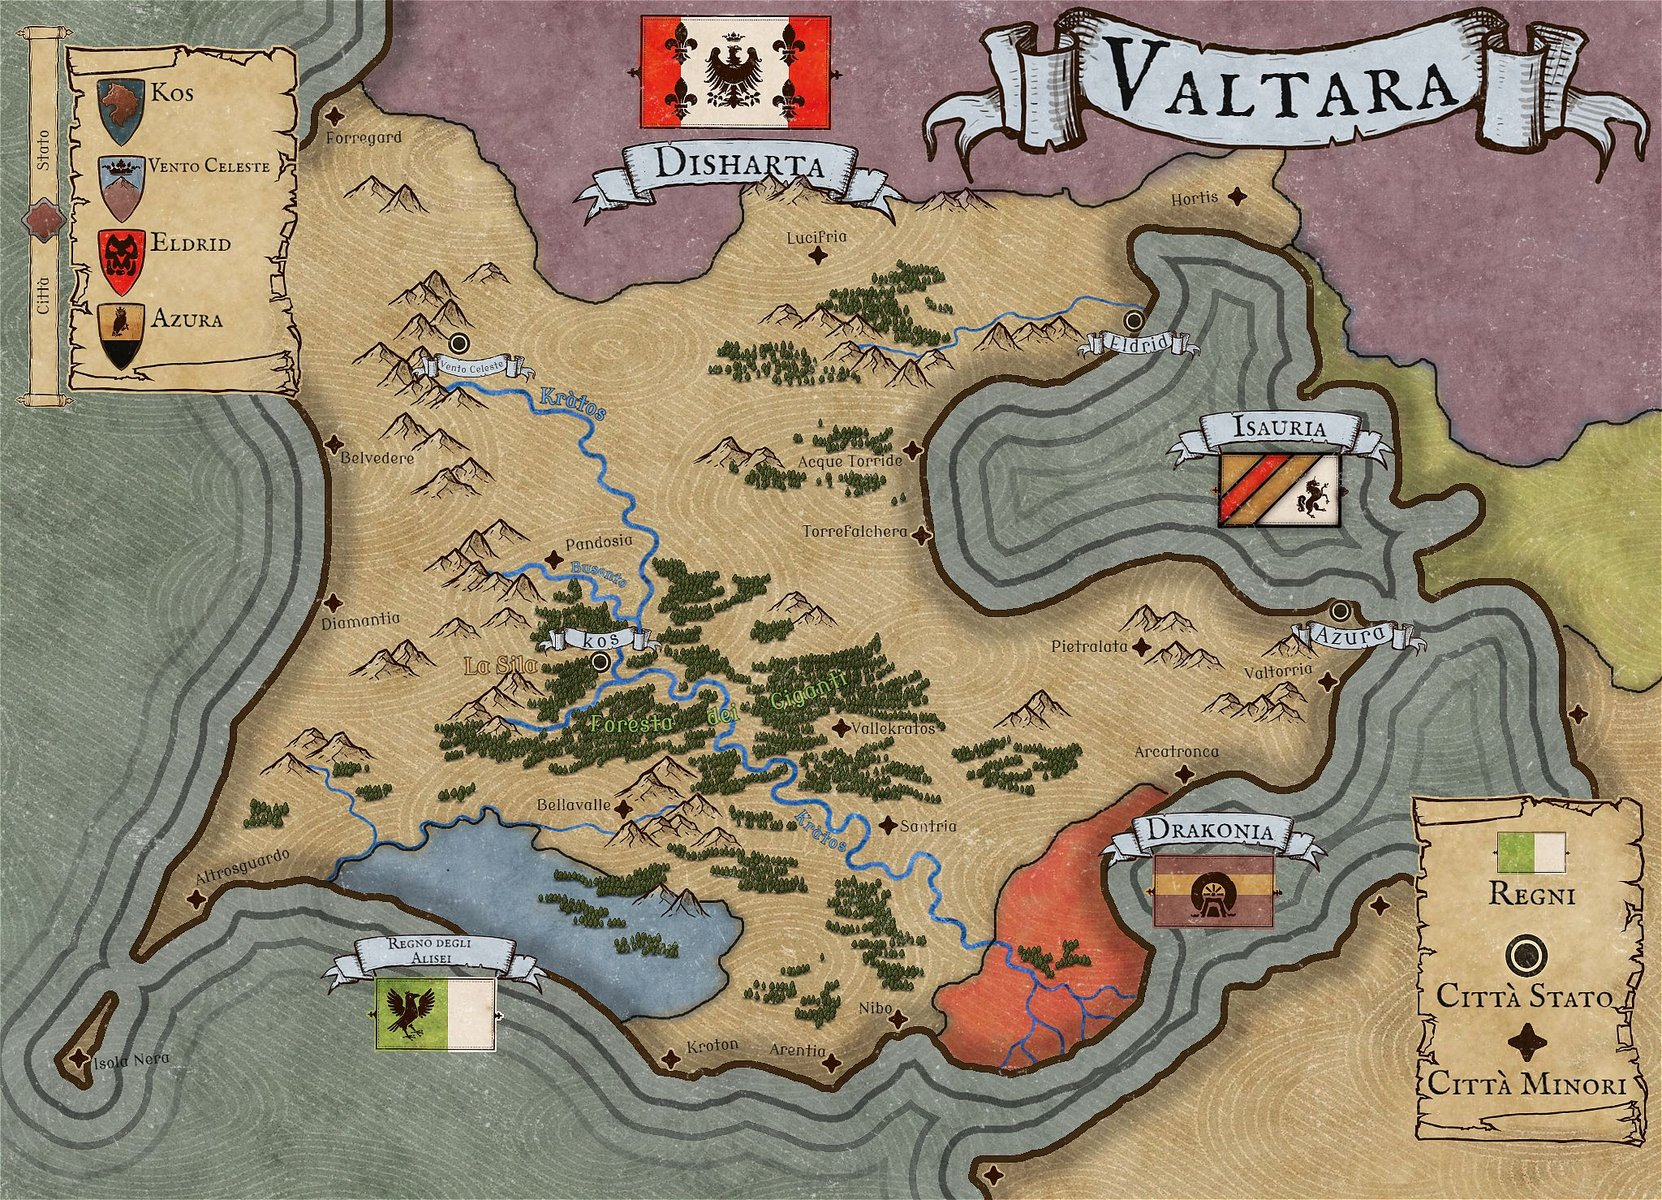
\includegraphics{Valtorria_2023.jpg}
\caption{Valtorria 2023.jpg}
\end{figure}
